% Chapter 1

\chapter{Introduction: A basis in fractal geometry} % Main chapter title

\label{Chapter1} % For referencing the chapter elsewhere, use \ref{Chapter1} 

\lhead{Chapter 1. \emph{Introduction}} % This is for the header on each page - perhaps a shortened title

%----------------------------------------------------------------------------------------

Before we discuss multifractals, we begin with a discussion of normal, or mono-fractals. We note the intuitive properties present in a simple example and how they differ from nonfractal geometry, and then 

%----------------------------------------------------------------------------------------
\section{An example of a fractal: the Koch snowflake (See Figure \ref{fig:kochcurve})}
\begin{figure}
\centering
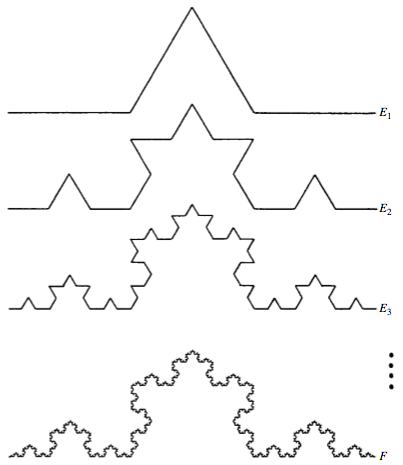
\includegraphics[scale=0.5]{Chapters/Figures/Kochcurve.png} 
\caption[Koch Curve]{Iterations of the Koch snowflake, a simple fractal exhibiting many characteristics typical of fractals. The straight line segment at the top is made more and more textured with each iteration $E_{n}$, becoming rougher and more fractal-like as it approaches the final Koch curve $F$. Image credit: \citep{fractaltextbook}. }\label{fig:kochcurve}
\end{figure}

We note the most obvious properties of this fractal that separate it from a non-fractal shape:
\begin{enumerate}
\item \textit{Its shape is defined recursively.} Each successive iteration replaces the middle third of each straight section with the two other sides of the equilateral triangle formed from that original third. This results in \textit{self-similarity} at all scales: any section of the Koch curve contains an infinite number of repetitions of the original curve.
\item \textit{Its length is not finite.} Because of the recursive rule defining the Koch curve, the curve's length is increased by a factor of $ \dfrac{4}{3} $ with each iteration. The total length can then be expressed as a geometric sequence with a common ratio of $ \dfrac{4}{3} $, which, because it is greater than one, will cause the sequence not to converge to a finite value. Other non-fractal approaches to the curve's characterization yield equally confusing results: the additional length added with each iteration expands the fractal's size in two dimensions, so one would expect to be able to classify the area in the plane that the curve fills. However, the curve's ``roughness'' is difficult to quantify with non-fractal geometry. This, as we will discuss below, leads to the creation of different \textit{fractal dimensions} to classify the space-filling properties of these fractals.
\item \textit{It has a fine structure.} The fractal has detail at all size scales, no matter how small\citep{fractaltextbook}.
\end{enumerate}


\section{Characterizing fractals}

As seen above, whereas non-fractal sets\footnote{We use the word ``set" to more precisely refer to what might be simply called a shape. After all, every shape is just a set, possibly infinite, of points.}  have well-defined, intuitively understood geometric properties such as length or area, fractal sets can be characterized by various concepts of dimension, most notably \textit{Hausdorff dimension}.

\subsection{Spaces, sets, and measures}

Before we venture further into classifying fractals by their dimension, we need to clarify a few definitions.

\newtheorem{mydef}{Definition}
\begin{mydef}
We define an n-dimensional space $ \mathbb{R}^{n} $ to be the set of all points that can be identified by an ordered n-ple of real numbers. Hence, for example, any point $ \alpha $ in $ \mathbb{R}^{5} $ can be identified by the ordered 5-ple $ \alpha = (\alpha_{1}, \alpha_{2}, \alpha_{3}, \alpha_{4}, \alpha_{5})$ where $ \alpha_{1} ... \alpha_{5} \in \mathbb{R} $.\end{mydef}

We will now work by analogy to discuss the concept of a \textit{measure}\footnote{Analogy adapted from \citep{mandelbrotmultifractal}}. Consider a geographical map of some landmass, with a function $ \mu(\mathcal{S}) $ that denotes the amount of groundwater below any subset $ \mathcal{S} $ of the landmass. We note three intuitive properties of this measure $ \mu $:
\begin{enumerate}
\item The measure of any subset of the space---or the amount of groundwater under any plot of land on the landmass---gives a numerical indication of the plot of land's magnitude. That is, it describes the plot's size when measured by groundwater content.
\item\label{measureofanullset} There should be no water under a plot of land with no size. 
\item\label{measureofsubsets} If a plot of land $ A $ contains another plot of land $ B $, there should be less or as much groundwater under $B$ as there is under $A$. 
\item\label{measureaddition} If we find the amount of groundwater under a plot of land on the landmass, we should get the same value or less than when we split the plot up into many pieces with overlap allowed and add up the amount of groundwater found under each piece. 
\end{enumerate}
We now formalize these properties below.

\begin{mydef}
We define a measure $ \mu $ to be a function on a space $ \mathbb{R}^{n} $ that assigns a positive number to each subset $ \mathcal{S} $ of $ \mathbb{R}^{n} $ such that:

{\addtolength{\leftskip}{10mm}
\begin{equation}
\mu(\emptyset) = 0
\end{equation}
Because $\mu$ should characterize a set by its size in some sense, it is meaningless to have a nonzero size for any set with no elements. This is reflected in Property \ref{measureofanullset} above.
\begin{equation}
\mu(B) \le \mu(A) \mathrm{ \quad if \quad }  B \subset A.
\end{equation} 
The size of a set should be smaller than (or equal to, if $ A = B $, i.e., $B$ is not a proper subset of $A$) the size of a set that contains the first set and other elements too. This is reflected in Property \ref{measureofsubsets} above.
\begin{equation}
\mu\left(\bigcup_{i=1}^{\infty} A_i\right) \le \sum_{i=1}^{\infty} \mu(A_i) 
\end{equation}

}

\end{mydef}

\section{And now multifractals too?}

\citep{mandelbrotmultifractal}






















